\documentclass[a4paper, 12pt]{report}
\usepackage{subfiles}
\usepackage[latin1]{inputenc}
\usepackage[english, danish]{babel}
\usepackage[T1]{fontenc}
\usepackage{amsmath,amssymb}
\usepackage{fancyhdr}
\usepackage{graphicx}
\usepackage{tabularx}
\usepackage{float}
\usepackage{color}
\usepackage{enumitem}
\usepackage{nameref}
\usepackage{caption}
\usepackage{pdflscape}
\usepackage{tabularx}
\usepackage{geometry}
\usepackage{titlesec, blindtext, color}
\usepackage{pdfpages}
\definecolor{gray75}{gray}{0.75}
\newcommand{\hsp}{\hspace{20pt}}
\titleformat{\chapter}[hang]{\Huge\bfseries}{\thechapter\hsp\textcolor{gray75}{|}\hsp}{0pt}{\Huge\bfseries}
\makeatletter
\newif\if@right
\def\shadequote{\@righttrue\shadequote@i}
\def\shadequote@i{\begin{snugshade}\begin{quote}\openquote}
\def\endshadequote{%
  \if@right\hfill\fi\closequote\end{quote}\end{snugshade}}
\@namedef{shadequote*}{\@rightfalse\shadequote@i}
\@namedef{endshadequote*}{\endshadequote}

\usepackage{url}
\usepackage{hyperref}

\newcommand\todo[1]{\textcolor{red}{TODO: }#1\PackageWarning{TODO:}{TODO tag!!}}


\makeatletter

\def\twodigits#1{\expandafter\two@digits\csname c@#1\endcsname}

\AddEnumerateCounter\twodigits\two@digits{01}


\makeatother




\fancyfoot[OC]{\textit{\thepage}}

\title{Sample title}
\date{\today}
\author{Asbj�rn Fjelbro Steffensen (afjs@itu.dk)\\ Thomas Stoy Dragsb�k (thst@itu.dk)\\ Nicki Hjorth J�rgensen (nhjo@itu.dk)\\ Jacob Benjamin Cholewa (jbec@itu.dk)\\ Jakob Merrild (jmer@itu.dk)\\ Mathias Kindsholm Pedersen (mkin@itu.dk)}

\begin{document}
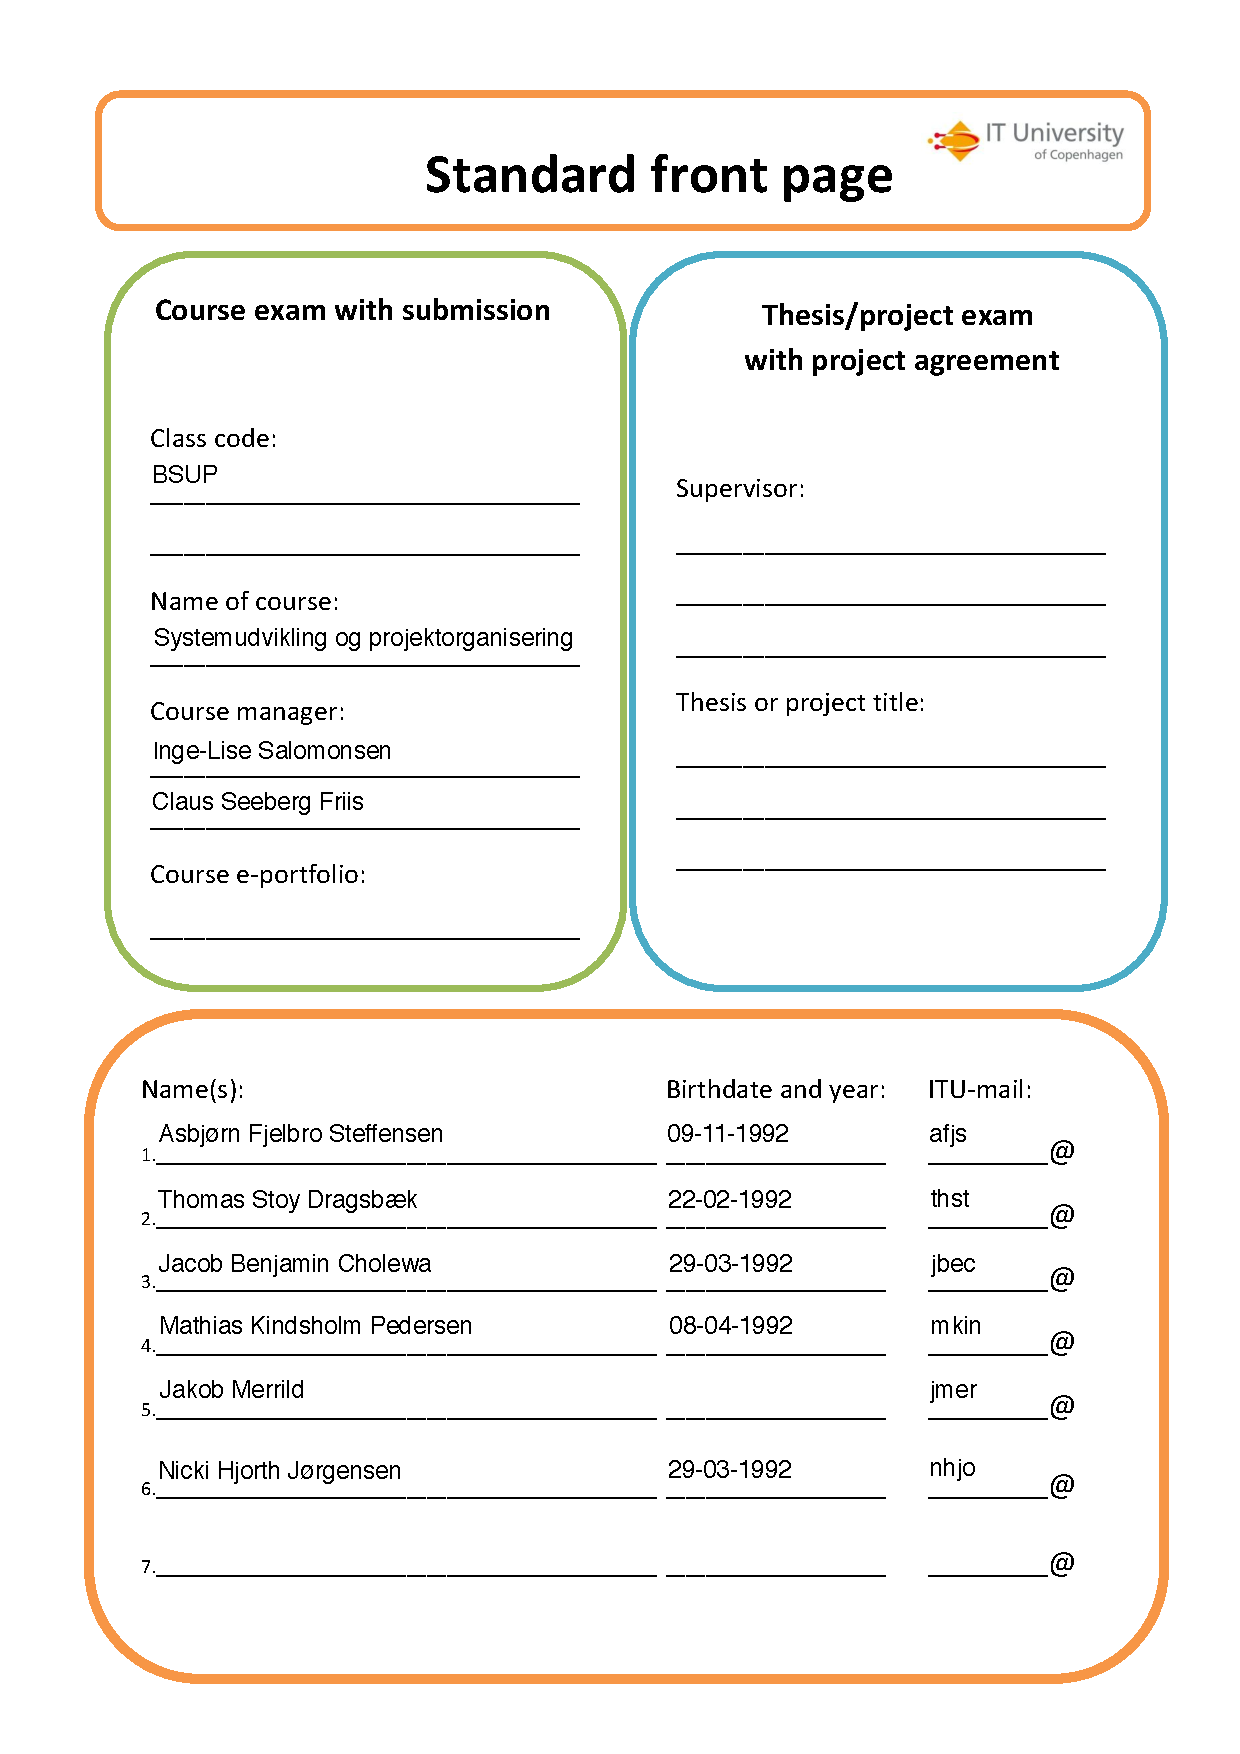
\includepdf{img/ituforside2.pdf}
\begin{titlepage}

\begin{center}

\topskip 7cm





\rule{\linewidth}{0.6mm}

\vspace{2mm}

\textsc{\LARGE Det gode eksamensprojekt og samarbejde} \\
\textsc{Systemudvikling og projektorganisering (BSUP)}
\vspace{1cm}
\rule{\linewidth}{0.4mm}

Asbj\o rn Fjelbro Steffensen (afjs@itu.dk)\\ Thomas Stoy Dragsb\ae k (thst@itu.dk)\\ Nicki Hjorth J\o rgensen (nhjo@itu.dk)\\ Jacob Benjamin Cholewa (jbec@itu.dk)\\ Jakob Merrild (jmer@itu.dk)\\ Mathias Kindsholm Pedersen (mkin@itu.dk)




\vfill

\large \today
\end{center}


\end{titlepage}

\newpage
\tableofcontents
\newpage

\chapter{Introduktion}
\subfile{tex/problemstatement.tex}
\newpage
\restoregeometry



\chapter{Aktivitetsplanl�gning}
I dette kapitel kigges der p� emner relevante for at svare p� f�rste sp�rgsm�l i problemformuleringen \\

\textit{1. Hvordan kan man planl�gge projektet?}\\

\noindent ved f�rst at kigge p� planl�gningen udf�rt i target-projektet og derefter p� precedence network som alternativ. 

\subfile{tex/productBreakdown.tex}
\newpage
\restoregeometry

\subfile{tex/activityBreakdown.tex}
\newpage
\restoregeometry

\subfile{tex/gantt.tex}

\subfile{tex/precedencenetwork.tex}
\restoregeometry

\subfile{tex/aktivitetsreflektioner}


\chapter{Estimering}
I dette kapitel analyseres forskellige estimeringsmetoder for at svare p� andet sp�rgsm�l i problemformuleringen \\

\textit{2. Hvordan kan man estimere hvor lang tid hver aktivitet i target-projektet tager?} \\

\noindent ved at unders�ge estimeringen udf�rt i target-projektet for derefter at se p� PERT og Use Case Points som alternativer.

\subfile{tex/planningpoker.tex}
\subfile{tex/PERT.tex}
\subfile{tex/useCasePoints.tex}
\subfile{tex/reflektion_estimering.tex}

\chapter{Procesmodeller}
\label{sec:procesmodeller}
I dette kapitel kigges der p� emner relevante for at svare p� tredje sp�rgsm�l i problemformuleringen \\

\textit{3. Hvordan kan man v�lge en passende procesmodel i target-projektet?}\\

\noindent ved f�rst at kigge p� procesmodellen brugt og derefter et alternativ.

\subfile{tex/scrumbut.tex}

\subfile{tex/waterfall.tex}

\subfile{tex/reflektion_procesmodel.tex}

\chapter{Diskussion}
%Which parts of the project could have been done differently for a better result?

\chapter{Konklusion}

\begin{thebibliography}{99}

\bibitem{hughescotterell09}
Bob Hughes and Mike Cotterell,
\textit{Software Project Management}.
McGraw-Hill Education,
5th Edition,
2009.

\bibitem{agilemanifesto}
Kent Beck, Mike Beedle and others,
\textit{Manifesto for Agile Software Development},
Sidst �ndret: 2001,
\url{http://agilemanifesto.org} (hentet 8. maj 2014)

\end{thebibliography}


\end{document}